\section{Method}

\begin{figure}
    \centering
    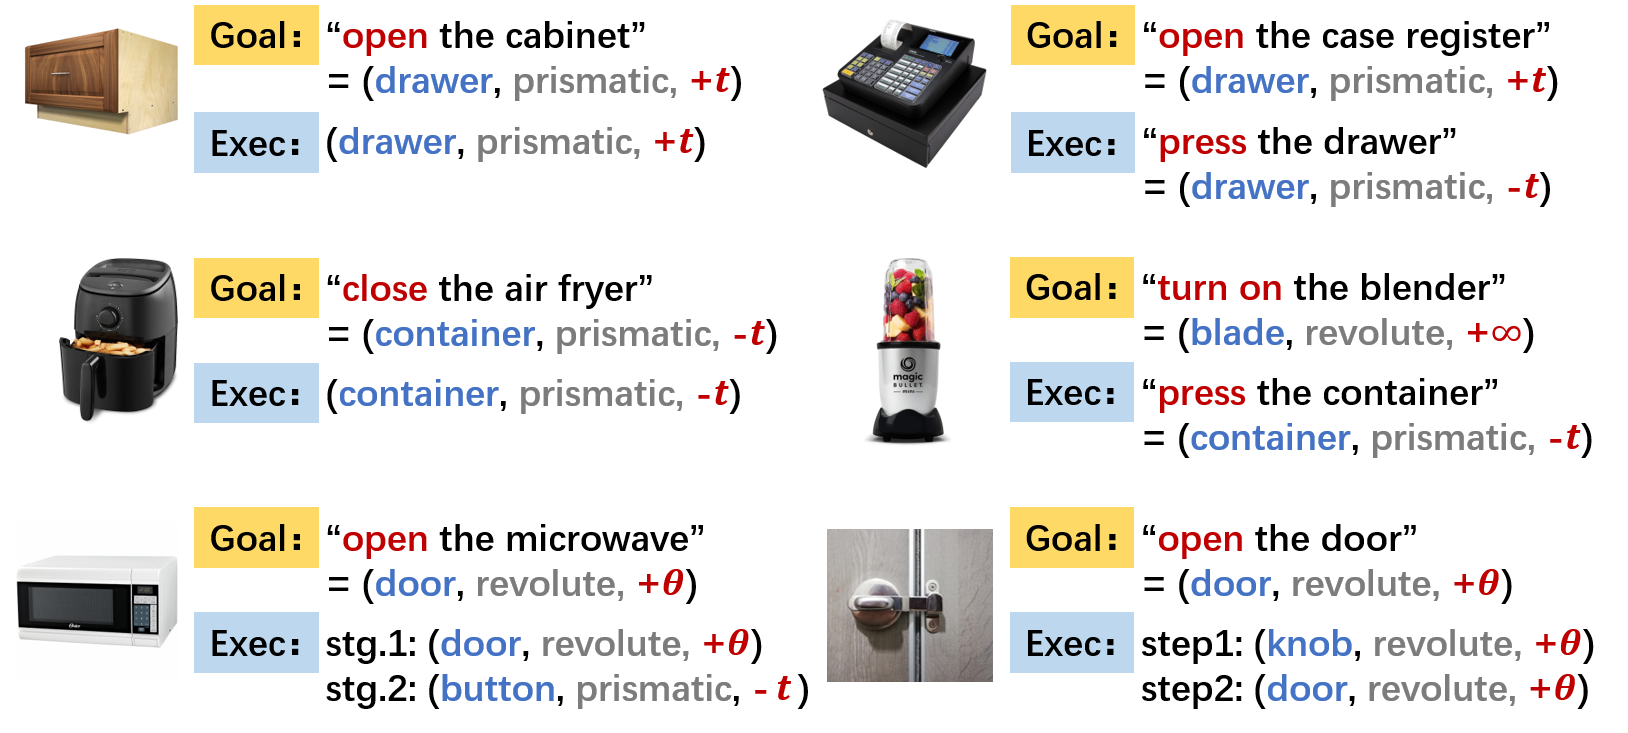
\includegraphics[width=\linewidth]{figures/tasks.png}
    \caption{\textbf{Objects, manipulation goals, and programmatic actions.}
    Each part-based action unit is represented as a 3-tuple of (part name, joint type, state change). Given the diverse structures and complex functionalities of the objects, the final action execution can be very different from the part state change directly implied by the input instruction.
    }
    \label{fig:tasks}
\end{figure}

% Pipeline detailed:
%         input: Language instruction; RGBD image
%         process: RGBD image --Segmentation model or Scene Caption Model(GAPartNet)-> {GAPart} detection --Heuristics-> Scene Description
%         LLM: prompt + Scene Description + Language Instruction --GPT4-> (semantic part, joint type, direction)
%         Perception: Semantic Part --GroundedSAM-> segmentation masks and dino feature --KNN Grounding-> GAPart Grounding
%         Skill: Predicted GAPart --GAPartNet-> Pose Estimation --Canonicalization-> Part\&Obj PointCloud with Dino Feature, Joint Type, Direction --I-PDF-> Start Point SE(3) Regression --SAPIEN-> Execution
    

% Our method seeks to implement human directives to guide a robot in performing complex and universally applicable manipulations of articulated objects. This section is structured as follows:
% (1) We present an overview of our methodological approach.
% (2) The procedure for processing human directives is explained.
% (3) The process of integrating visual observation with processed language parts to form interaction information is elucidated.
% (4) We describe the procedure for executing specific skills and accomplishing predefined tasks.

% \TODO{A brief problem formulation}
Our tasks revolve around language-guided manipulation of articulated objects. Given a natural language instruction, denoted as $\tilde{I}$, the robot is expected to generate a precise and appropriate manipulation trajectory to complete the given tasks. It is important to note that the natural language instruction $\tilde{I}$ may be subject to ambiguity and extreme diversity, and the articulated object may have certain joint constraints or intricate structures (Fig. \ref{fig:tasks}). Therefore, it necessitates both semantic understandings of object functionalities as well as physically plausible executions for successful task completion.

%In this section, we present our framework for such language-guided articulated object manipulation. This approach takes articulated object manipulation instructions, RGBD images, and optionally, supplementary information such as an object manual as input. The primary stage of our process engages a context-aware instruction interpreter to systematically process and analyze both language and visual input, see \ref{language_method}. We integrate scene descriptions derived from visual inputs with a Visual-Language Module (VLM) that include instructions and additional data to formulate a prompt for the Large Language Model (LLM). This subsequently yields a structured format delineating interaction strategies and procedural steps. Following this, we present our part manipulation generation module that utilizes the cognitive module's output as its input, see \ref{policy_method}. The first step involves grounding the part within the articulated system to be manipulated, referring to this as GAPart. Subsequently, using an innovative probabilistic manipulation proposal model, we generate an appropriate manipulation strategy\TODO{More details here?}

\subsection{Context-Aware Instruction Interpreter}
\label{language_method}
%\TODO{instruction? vision description? a part of instruction?}
%\TODO{input format: instruction, scene description(optional?), manual(optional)}

\paragraph{Action programs}
The goal of the instruction interpreter is to translate natural-language instruction $\tilde{I}$ into programmatic instructions.
We define the most basic manipulation on one single part of articulated objects as an ``action unit'', which can be represented by a 3-tuple $\va = (\tilde{p}, j, \Delta s)$ with part name $\tilde{p}$, joint type $j$, and the change of part state $\Delta s$.
The part name $\tilde{p}$ is a noun in natural language which will later be sent into an open-vocabulary segmentation module; $j$ refers to the joint directly linked to part $\tilde{p}$ and indicates whether it is a revolute or a prismatic joint; $\Delta s$ is the state change of joint $j$ under the action, which is either an angle $\pm\theta$ if $j$ is revolute or a relative translation $\pm t$ \wrt the part bounding box if $j$ is prismatic.
%
The final output of the interpreter should be in one of the following formats:
\begin{itemize}
    \item a single action unit,
    \item an unordered union of multiple action units,
    \item an ordered list of multiple action units,
\end{itemize}
or be a finite combination of the three formats.
%
Following the convention of programming languages (PL), this can be viewed as a typing system with expressions:
\begin{equation*}
    \va ~|~ \texttt{Union}\{\va,\va\} ~|~ \texttt{List}[\va,\va]
\end{equation*}
Here the \texttt{Union} expression is for non-deterministic policy generation when multiple action units can reach the same goal, e.g. in Fig. \ref{fig:tasks} bottom left, both pulling the door and pressing the button results in the microwave door being opened.
\texttt{List} is for sequential action generation when no single-step solution exists, e.g. in Fig. \ref{fig:tasks} bottom right, in order to open the door, the knob must be first rotated to unlock the door.


\begin{figure}
    \centering
    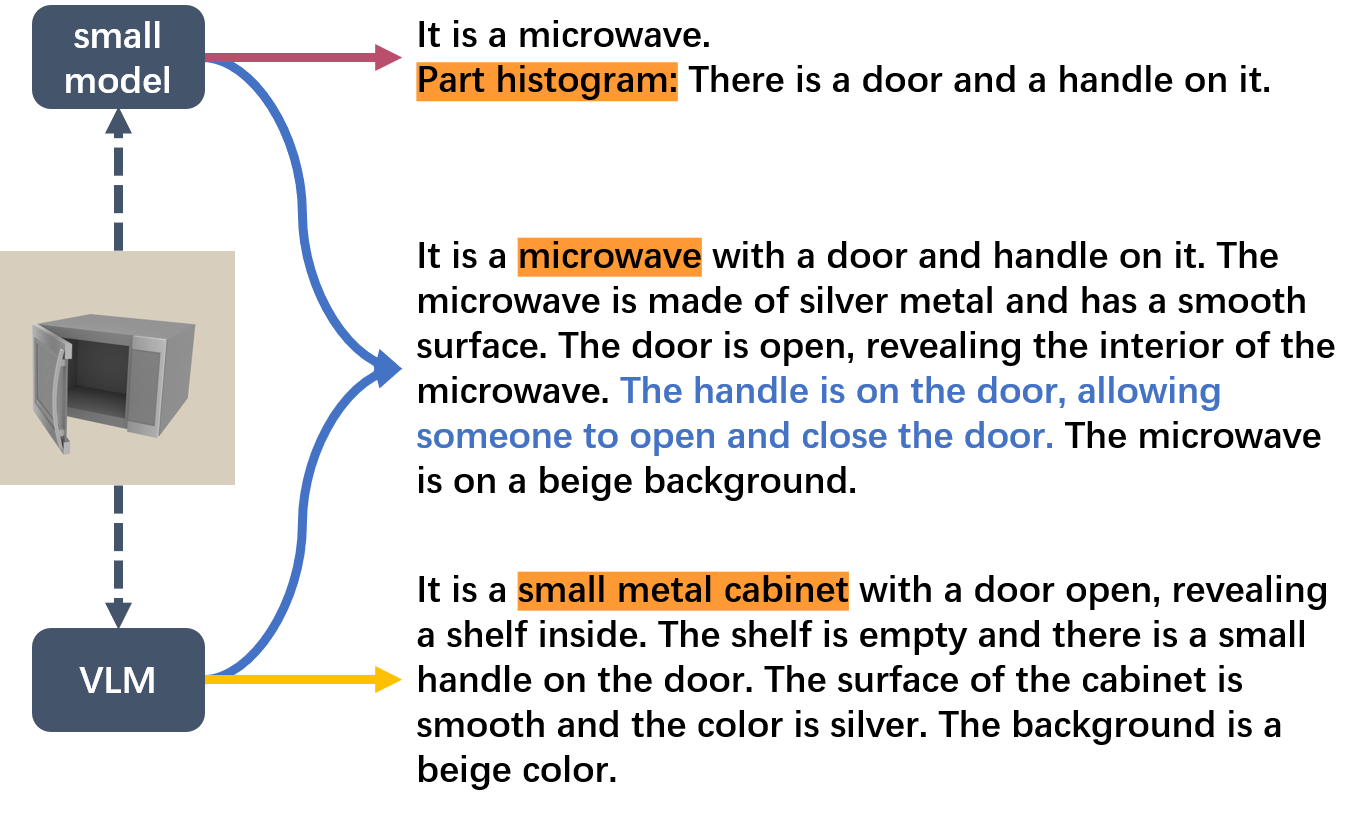
\includegraphics[width=.9\linewidth]{figures/scene_context_parser.png}
    \caption{\textbf{Scene context parser.}
    \textbf{Top:} The small perception model provides accurate histograms of actionable parts in a plain style.
    \textbf{Bottom:} Large VLM generates rich text but is less accurate.
    \textbf{Middle:} Combining the two models facilitates the generation of informative descriptions with better correctness and task relevance.
    }
    \label{fig:scene_context_parser}
\end{figure}

\paragraph{Input parsing}
We employ a Large Language Model (LLM) to parse the input instruction, which outlines the intended goal. 
To ensure our model is cognizant of the scene context, we incorporate a Visual-Language Model (VLM) to interpret the visual inputs and procure a language description of the scene.

Specifically, drawing inspiration from \cite{greff2020binding}, we recognize that the inclusion of expert facts can enhance the correctness of visual perception. Thus, we first extract an actionable part histogram using a small segmentation model from \cite{geng2022gapartnet}, and pass it into the VLM together with the task description to generate a comprehensive scene description.
By enforcing coherence between the expert knowledge of the small model and the general knowledge of the large model, we can acquire scene descriptions that are more accurate and also task-related (Fig. \ref{fig:scene_context_parser}).
More prompt details can be found in \SupplementaryMaterial.


Here shows an example of the overall inputs and outputs of the instruction interpreter:

\vspace{.5ex}
\noindent\fbox{\parbox{0.97\linewidth}{\scriptsize{\texttt{% <-- removes unnecessary first line indent
{\color{blue}Input:}\\
Open the microwave. \\
Scene description: It is a microwave with a door and handle on it. The microwave is made of silver metal and has a smooth surface. The door is open, revealing the interior of the microwave. The handle is on the door, allowing someone to open and close the door. The microwave is on a beige background. \\
{\color{blue}Output:} \\
Strategy 1: 1 step: (1) (Door, revolute, +90) \\
Strategy 2: 1 step: (1) (Handle, revolute, +90) \\
Strategy 3: 2 steps: (1) (Button, prismatic, -0.5) (2) (Door, revolute, +60) \\
Strategy 4: 2 steps: (1) (Handle, revolute, +30) (2) (Door, revolute, +60)
}}}}
\vspace{.5ex}

Certain objects such as appliances have very diverse and intricate structures that can hardly be covered by general knowledge priors. Therefore, we also accommodate the additional input of the object usage manuals, which can be easily accessed together with the purchase of the object in real-life applications. This feature allows the LLM to gain expert knowledge of the object and thereby provide more precise and relevant outputs.

\vspace{.5ex}
\noindent\fbox{\parbox{0.97\linewidth}{\scriptsize{\texttt{% <-- removes unnecessary first line indent
{\color{blue}Input:}\\
Turn on the blender. \\
Scene description: It is a blender with a clear lid on it. The blender is made of stainless steel and has a black base. \\
User manual: \\
-Usage: \\
--1. Fill the blender cup with the ingredients. \\
--2. Press the lid to start blending, and release to stop. \\
--3. Stop blending and unplug the power. \\
-Maintenance: \\
--1. Clean immediately after use. \\
--2. Be cautious of the sharp blade. \\
--3. Store in a dry, cool place after drying.\\
{\color{blue}Output:} \\
Strategy: 1 step: (1) (Lid, prismatic, -0.5)
}}}}
\vspace{.5ex}

Throughout our usage of the LLM, we have carefully designed prompts of output format descriptions and also a small number of success and failure cases to better guide the LLM. Details can be found in the \SupplementaryMaterial.


%\TODO{manualupdate}
%To elucidate how the instruction interpreter operates, let's consider an example. We initially accept human instruction as input, for instance, "Turn on the blender". Optionally, we also provide scene descriptions like "There is a lid on it" and a manual that could read "Please first press the lid and the machine will work."

%These instructions are assimilated into the prompt and processed by the GPT-4 language model. The model subsequently produces the output in a formal format. An example of such output could be "Strategy: 1 step: (1) (Lid, prismatic, -0.5)".

%In this instance, the language model identifies the critical semantic parts $\tilde{p}$ within the articulated object that is necessary for the successful execution of the given task (for example, the "lid"). The joint type $j$ conveys the motion paradigm; for instance, "prismatic" implies the need to move the robot hand parallelly along the axis of the joint. Lastly, the part target state $\Delta s$ symbolizes the direction and distance or angle of the manipulation.
%\TODO{}It's important to note that angles are absolute, whereas distances are relative and pertain to the ratio of relative axis lengths.
% Here we give an example to illuminate how the instruction interpreter works. We first take human instruction as input, (\eg Turn on the blender). Then optionally, we also provide scene descriptions (\eg There is 1 lid on it.) and manual (\eg Please first press the lid and the machine will work.).
% These instructions are integrated into the prompt and processed by the GPT-4 language model. 
% Then the model output the formal format output, such as Strategy: 1 step: (1) (Lid, prismatic, -0.5). Here the language model identifies the semantic parts $\tilde{p}$ within the articulated object that is essential for the successful completion of the given task (\eg lid). The joint type $j$ explains the motion paradigm, for example, prismatic means we need to Parallel move the robot hand along the axis of the joint. And the part target state $\Delta s$ represents the manipulation direction and distance or angle. Here angles are absolute and distances are relative and refer to the ratio of relative axis lengths. 



% For instance, given an instruction $I = \text{"Please open the cabinet"}$, GPT-4 identifies and communicates that semantic parts such as "handles", "knobs", "doors", "hinges", "locks", and "drawers" are essential for executing the task. This interpretation occurs without requiring any additional specification.



\subsection{Part Manipulation Generator}
\label{policy_method}

\begin{figure}
    \centering
    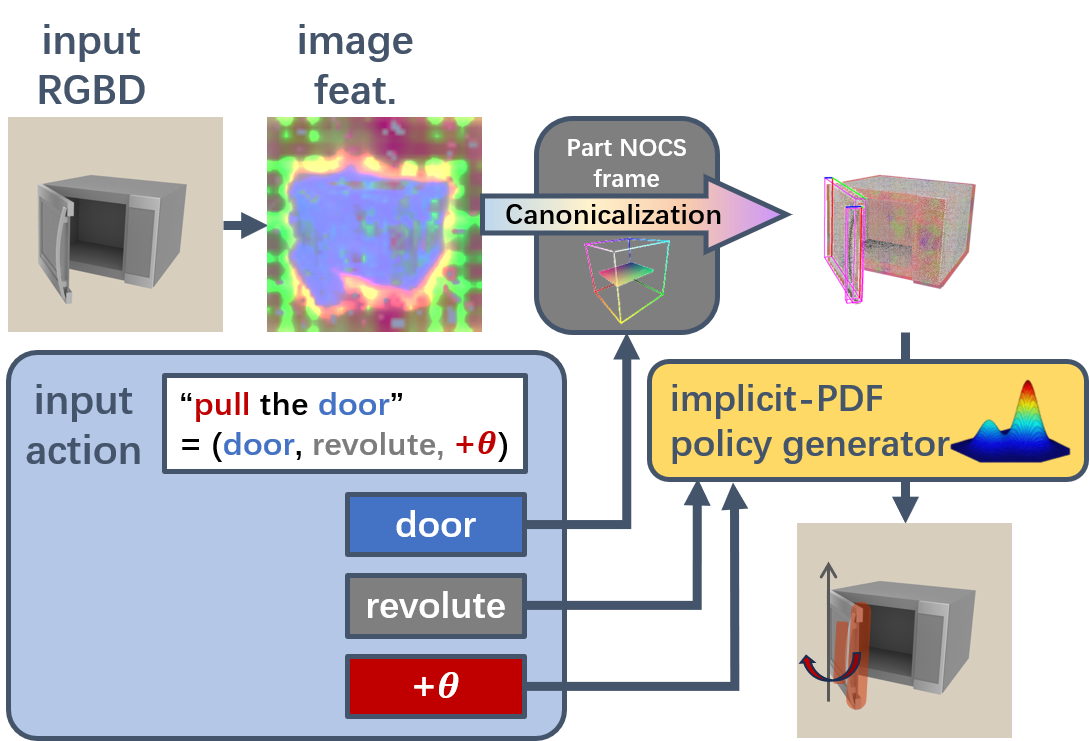
\includegraphics[width=.9\linewidth]{figures/part_manip_generator.png}
    \caption{\textbf{Part manipulation generator.\todo{REPLACE}}
    }
    \label{fig:part_manip_generator}
\end{figure}

Given an action unit $\va = (\tilde{p}, j, \Delta s)$, the part manipulation generator turns it into gripper trajectories that can be executed by a robot arm.

\paragraph{Part perception}
Given an RGBD image observation $\vo$, we first apply an open-vocabulary object segmentation model \cite{kirillov2023segany,liu2023grounding} to identify the semantic part $p$ queried by $\tilde{p}$ and extract the DINO features \cite{oquab2023dinov2} of the part in the image space.
Then, using the pose estimation module for \cite{geng2022gapartnet}, we obtain the pose $\rmT = (\rmR, \rvt)$ and the Normalized Object Coordinate System (NOCS) for part $p$ and canonicalized part feature $F^{\text{canon}}_{\text{part}}$ and the object feature $F^{\text{canon}}_{\text{object}}$.
As the pose estimator is trained on GAParts, it shows strong generalizability across different object categories.

%Notice that the GAPart definition\cite{geng2022gapartnet} serves as a bridge, creating a link between the semantic-centric and the manipulation-centric representation of the articulated object.

%Upon having the RGBD image and the segmented part $\tilde{p}$ as input, we subsequently utilize the GAPart Perception Module. The module's initial task is to ground the segmented semantic part to a GAPart class, following which it estimates the pose of this part. We get the predicted GAPart $p$ and corresponding pose $\rmT$.

\paragraph{Policy generation}
Given the predicted GAPart $p$, part poses $\rmT$, manipulation joint type $j$, and target part state $\Delta s$, our next step is to generate an interaction policy to accomplish the task. 

Due to the multi-ground-truth nature of possible manipulation policies for a certain part, we utilize a probabilistic model called implicit-PDF \cite{implicitpdf2021} to generate the probability distribution of policies to sample from instead of directly predicting one single policy. We start this process by employing a probabilistic \textbf{SE}(3) estimator
\begin{equation*}
    p(\,\cdot\,|\, F^{\text{canon}}_{\text{part}}, F^{\text{canon}}_{\text{object}}, \Delta s):
    \textbf{SE}(3) \rightarrow \R^{+}
\end{equation*}
%
on the initial robot hand pose $\rmT_{\text{hand}}$. The input of this module includes: part feature $F^{\text{canon}}_{\text{part}}$, object feature $F^{\text{canon}}_{\text{object}}$, GAPart Pose $\rmT$, and target part state direction $\Delta s$. %We first canonicalize the part feature and object feature with the predicted part pose. Taking these features and directions as input, we estimate the initial robot hand pose likelihood.

To train the probabilistic policy generation module, we gather a collection of initial hand poses, features, and target states from successful manipulation trajectories, denoted as  $(F^{\text{canon}}_{\text{part}}, F^{\text{canon}}_{\text{object}}, \Delta s, R_0, t_0)$, and optimize for the network parameters with the loss: 
\begin{align*}
    &\gL(F^{\text{canon}}_{\text{part}}, F^{\text{canon}}_{\text{object}}, \Delta s, R_0, t_0) \\
    &= -\log(p(R_0, t_0| F^{\text{canon}}_{\text{part}}, F^{\text{canon}}_{\text{object}}, \Delta s))
\end{align*}
%
\TODO{Compute trajectory from the initial gripper pose, part joint structure, and $\Delta s$.}

%\begin{algorithm}
%    \caption{Part Manipulation Generator}\label{algo_part_manip}
%    \hspace*{\algorithmicindent} \textbf{Input} action unit $\va = (\tilde{p}, j, \Delta s)$, RGBD observation $\vo$ \\
%    \hspace*{\algorithmicindent} \textbf{Output} execution result
%    \begin{algorithmic}[1]
%        \STATE $F^{\text{canon}}_{\text{part}}, F^{\text{canon}}_{\text{object}} = percept(\va, \vo)$ \COMMENT{Part Perception}
%        \FOR{epochs = $1$ to $N$}
%            \WHILE{$(j\le m)$}
%                \STATE Randomly initialize $w_i=\{w_1,w_2,\dots,w_n\}$
%                \STATE input $o_j=\{o_1,o_2,\dots,o_m\}$ in the input layer
%                \STATE forward propagate $(f_i\cdot w_i)$ through layers until getting the predicted result $y$
%                \STATE compute $e=y-y^2$
%                \STATE back propagate $e$ from right to left through layers
%                \STATE update $w_i$
%            \ENDWHILE
%        \ENDFOR
%    \end{algorithmic}
%\end{algorithm}

\begin{algorithm}
    \caption{Part Manipulation Generator}\label{alg:part_manip}
    \begin{algorithmic}[1]
    \Require action unit $\va = (\tilde{p}, j, \Delta s)$, RGBD observation $\vo$ % input
    \Ensure execution result % output
    \State $F^{\text{canon}}_{\text{part}}, F^{\text{canon}}_{\text{object}} = percept(\va, \vo)$ \Comment{Part Perception}
    \State $\rmT_{\text{hand}} = \Argmax{p(\,\cdot\,|\, F^{\text{canon}}_{\text{part}}, F^{\text{canon}}_{\text{object}}, \Delta s)} $
    \State trajectory $\tau = heuristic(\va, \rmT_{\text{hand}})$ \Comment{Policy Generation}
    \State execute $\tau$ with a physical agent 
    \end{algorithmic}
\end{algorithm}

%With the comprehensive definition and annotation facilitated by GAPartNet\cite{geng2022gapartnet}, we have the ability to query the manipulation joint directly from the GAPart pose. It's noteworthy to mention that the manipulation strategies for articulated parts are specific to their structure. For instance, a part with a revolute joint should ideally move along the axis of revolution.

%Given these unique characteristics, we create specific heuristics to generate trajectories for different joint types, enabling us to manipulate the parts more effectively and accurately. To illustrate this, consider a door with a revolute joint that needs to be opened 60 degrees. We would initially predict the hand-grasping pose $\rmT_{hand}$. During the interaction phase, the pose of the hand is rotated 60 degrees along the axis to successfully complete this manipulation step.

% Given the predicted GAPart $p$, Part poses $\rmT$, manipulation joint type $j$, and target part state $\Delta s$, we then generate an interaction policy to finish the task.
% We first introduce a probabilistic SE(3) estimator to estimate a suitable initial grasping pose. Thanks to the universal definition and annotation of GAPartNet, we can query the manipulation joint from the GAPart pose. Notice that the articulated parts have certain manipulation strategies, for example, for a revolute joint, the part should move along the revolute axis. So for different joint types, we design certain heuristics to manipulate the parts. 

% Finally, we implement the grounded manipulation policy, represented as $\pi$, to accomplish the task. This policy requires additional input data, specifically the part pose, which we denote as $\text{POSE}$. $\text{POSE}$ is obtained using a trained pose estimator. The pose estimator provides sufficient information for the policy to guide the robot toward task completion.

% This general methodology ensures that the robot is capable of executing a wide range of tasks involving the manipulation of articulated objects, using natural language instructions and visual observations. The grounding of semantic elements to physical parts of the object, combined with the optimal manipulation policy, guides the robot's actions in response to a variety of tasks.

% \todo{double check and write I-PDF part}

% \section{Method}
% In general terms, we utilize innate human directives to facilitate the execution of a robot's intricate and universally applicable manipulations of articulated objects. This segment is structured as follows:
% (1) We present an overview of our methodological approach.
% (2) The procedure for processing intrinsic human directives is explained.
% (3) The process of integrating visual observation with processed language parts to form interaction information is elucidated.
% (4) We describe the procedure for executing specific skills and accomplishing the predefined tasks.
% \subsection{Overview}
% \haoran{add degree?}
% Our system for manipulating articulated objects starts by taking human instructions as its initial input. We seamlessly integrate this instruction into our system prompt, which is then processed by GPT-4. The AI determines the semantic elements within the articulated object that are capable of completing the given task. This includes deciding whether the specific part should be distanced from or drawn closer to the object to execute the task effectively—essentially, whether the joint should be opened or closed, and if it needs to be specified to what extent in the instruction.

% For instance, if the instruction is "Please open the cabinet", GPT-4 will identify and communicate that parts such as "handles", "knobs", "doors", "hinges", "locks", and "drawers" are crucial for this task, without any additional specifics required.

% Utilizing the outputs from GPT-4, we input the semantically identified parts into Grounded SAM (GroundingDINO + SAM)\cite{kirillov2023segany,liu2023grounding}, yielding the segmented parts and the DINO visual feature. We then employ a max-pooling operation to extract the part-specific DINO feature and utilize KNN (K-Nearest Neighbors) to ground the semantic part to the GAPart definition. This grounding process bridges the gap between visual perception and the manipulation-centric GAPart definition.

% Following the GAPart embedding, we proceed to embed the manipulation policy into the current observational context. Here, we leverage KNN once more to identify the nearest part and the corresponding optimal manipulation policy (the one with the highest success rate for manipulation).

% Subsequently, we adhere to the grounded manipulation policy to accomplish the task. This policy requires additional input data, specifically the part pose, which is obtained using our trained pose estimator. This estimator supplies sufficient information for the policy, thereby facilitating task completion.


% \subsection{Language Processing and Prompts for LLM}
% \haoran{Symbols and formulas}

% The large language model (LLM) processes the human directives and generates semantically understandable instructions that our GAPart grounding system can interpret. This task involves identifying key phrases or parts within the directives and then assigning the appropriate manipulative action to each specified part of the articulated object. GPT-4, the underlying language model, serves this crucial purpose.

% The human instructions are formulated into a structured system prompt, which the GPT-4 model then processes. Our detailed prompt can be found in the supplementary materials. By analyzing the instruction, GPT-4 identifies the semantic parts and defines the specific manipulations necessary to accomplish the task. This system helps to determine the necessary parts and the manipulation policy without the need for explicit user instructions.

% $$\{\text{Semantic Parts}\}, \{\text{Manipulation Info}\} \leftarrow \text{GPT--4} (\text{Prompt Template}(\text{Human Instruction}))$$


% \subsection{Joint Embedding of Semantic and Actionable Parts}
% After processing the language parts and identifying the semantic parts, we merge these findings with visual observations from an off-the-shelf Foundation Model, Grounded SAM\cite{}. This fuses the semantic information with the object's visual characteristics, forming a comprehensive representation of the task.

% The outputs from GPT-4 are inputted into Grounded SAM, which segments the object's parts and determines the corresponding DINO visual feature. We then perform a max-pooling operation to extract part-specific DINO features. Utilizing K-Nearest Neighbors (KNN), we ground the semantic part to the GAPart definition, thereby bridging the gap between the semantic understanding and the Generalizable Part definition, which makes the downstream manipulation easier.
% \todo{details}

% Following this, we use a similar way to embed the manipulation policy into the observational context. This involves finding the nearest part and determining the corresponding optimal manipulation policy.

% \todo{details}



% \subsection{Action Execution}
% Once the manipulation policy is defined and embedded within the current context, the robotic system proceeds to carry out the task. It leverages the grounded manipulation policy and additional input data to perform the necessary actions. The additional data comprise the part pose, which is obtained using our trained pose estimator.

% This pose estimator provides the system with the exact orientation and location of the object part. This crucial information is needed for the manipulation policy to guide the robot's actions accurately and effectively. Thus, by combining the grounding of semantic understanding, actionable parts, and the current observational context, the robot successfully accomplishes the task.




